%!TEX output_directory = .aux
%!TEX copy_output_on_build(true)

\documentclass[11pt,a4paper, titlepage]{article}
\usepackage[a4paper, total={6.5in, 8in}]{geometry}
\usepackage[utf8]{inputenc}
\usepackage{amsfonts}
\usepackage{amssymb}
\usepackage{amsmath}
\usepackage{mathtools}
\usepackage{forest}
\usepackage{subfig}
\usepackage{natbib}
\usepackage{etoolbox}
\usetikzlibrary{shapes.geometric,positioning, arrows,trees, positioning, fit, calc}
\tikzset{circ/.style={circle,draw, solid, inner sep=0pt,minimum size=10mm}}
\usepackage{amsthm}
\usepackage{setspace}
\usepackage[hidelinks]{hyperref}
\usepackage{cleveref}

\doublespacing

\title{An Analysis of Smart Voting in Liquid Democracy}
\author{Student: 1033308}
\date{\today}
\newtheorem{theorem}{Theorem}
\newtheorem{prop}[theorem]{Proposition}
\newtheorem*{remark}{Remark}
\DeclarePairedDelimiter\abs{\lvert}{\rvert}
\DeclarePairedDelimiter\norm{\lVert}{\rVert}


\theoremstyle{definition}
\newtheorem{definition}[theorem]{Definition}
\newtheorem{example}[theorem]{Example}
\newtheorem{corollary}[theorem]{Corollary}
\newtheorem{lemma}[theorem]{Lemma}
\newtheorem{proposition}[theorem]{Proposition}
\newtheorem*{idea}{Idea}

\crefname{definition}{Definition}{Definitions}
\crefname{figure}{Figure}{Figures}
\let\vec\mathbf

% MACROS
\newcommand{\BMM}{\textsc{BoundedMinMax}}
\newcommand{\BMS}{\textsc{BoundedMinSum}}
\newcommand{\BMMS}{\textsc{BoundedMinMaxSum}}
\newcommand{\Maj}{\mathit{Maj}}
\newcommand{\LIQUID}{\mathit{LIQUID}}

\begin{document}

\begin{titlepage}
    \begin{center}
        \huge
        \textbf{The Limits of Smart Voting in Liquid Democracy}

        \vfill
        
        
\includegraphics[width=0.35\textwidth]{logo.jpeg}
        
        \vfill
        
        \LARGE
        Student: 1033308 \\
        \Large
        Supervisor: Edith Elkind\\
        
        \vspace*{1.5cm}
        
        4\textsuperscript{th} Year Project Report\\
        \vspace*{2pt}
        Honour School of Mathematics and Computer Science (Part C)\\
        \vspace*{.5cm}
        Trinity Term 2022 \\
        Words: 9917
    \end{center}

\end{titlepage}

\renewcommand{\abstractname}{Acknowledgements}
\begin{abstract}
    I begin by acknowledging the guidance of my supervisor Edith Elkind. Without her exceptional knowledge of recent academic developments, insightful comments and the time she dedicated to reviewing my manuscript this work would not be possible.
For this, I am extremely grateful.

Further, I am very appreciative to the hours my tutors have spent to sharpen my mind in the last four years. I'm grateful to them for helping me blossom to the student I am today.

I want to thank my good friends for taking the time to look through my work and for bouncing off ideas about a solution that never came to be.
I wish I could thank my tutors and friends by name, but guidance from the academic office forbids me to do so.

Finally, I want to thank my family for the support throughout my life and especially this last year.

\end{abstract}

\newpage

\tableofcontents

\newpage

\section{Introduction}

Liquid democracy, also referred to as delegative democracy, is a decision-making mechanism that allows greater choice to voters than representative democracy.
Firstly, every voter is allowed to vote directly on an issue. 
Voters can delegate their vote to other voters.
Importantly delegations are \emph{transitive}. 
So we allow Alice to delegate to Bob and Bob to delegate to Charlie. In this case Charlie votes with the combined power of all three.

One of the first published proposals of this model is a non-technical work by \cite{ford2002delegative}. 
Ford claims that large-scale direct democracy is infeasible and likely undesirable.
It is infeasible because of the frequency of policy decisions and likely undesirable because the ``effective wisdom of the collective can easily turn out to be much worse than its average.''
Representative democracy on the other hand, holds elections every so often. Winners get to represent their constituency while losers gain no representative power.
Additionally, there is a prescribed limit on the total number of elected representatives and every voter can pick from a limited number of representatives.

Delegative democracy is introduced as a balance of the two by challenging the premise that the number of representatives needs to be kept small.
In this model, voters that wish to do so, can vote directly on issues.
Passive voters can delegate to the representatives called delegates.
Delegates are not chosen through time-specific elections but need to canvas voters continually.
When delegates vote, they vote with the combined power of all voters that delegate for them.
They can vote on issues directly, or they can delegate to other more specialised delegates.
A key idea is that delegates need not win competitive elections and that delegates have their votes made public for the sake of accountability. 
Ford then introduces notions to replace the parliamentary committees in a setting of liquid democracy.
Then, Ford introduces strengthenings of liquid democracy.
Of interest is the ability to split votes, where agents can delegate fractions of their votes to different delegates. 
Even more interesting is that Ford introduces the ability of agents to submit ``multiple delegation choices in order of preference.'' This is done partly to deal with the case of cycles, where Alice delegates to Bob but also Bob delegates to Alice.
This is one of the key extensions of Liquid Democracy we consider in our work.

\subsection{Liquid Democracy and Ground Truth}
An important strand of work in Liquid Democracy is to have Liquid Democracy find a ground truth. 
A key contribution is by \citet{kahng2021liquid}. 
The model considers binary issues $\{0, 1\}$ with $0$ being the incorrect outcome and $1$ being the correct outcome. Every voter $i$ has a competence level $0 \leq p_i \leq 1$, which is the probability that a direct vote of voter $i$ is a correct vote.
Further, voters are only able to pick delegators from a predefined social network. This can be thought of as a directed graph.
These delegates are called the neighbours of $i$.
Further, agents are only allowed to delegate to agents that are more competent than them by some global constant $\alpha >0$.
So, voter $i$ may delegate to their neighbour $j$ if and only if $p_i + \alpha \leq p_j$. 
We say that $i$ approves of $j$.
This rules out the problem of cyclical delegations a priori, as $\alpha > 0$.

Delegation mechanisms in this context are functions which input an instance of the model and output, for each voter $i$, a delegation probability distribution over the agents $i$ approves of.
Then the majority rule is applied on the outcome of a delegation mechanism. Ties are broken arbitrarily.
The probability that the group votes for the correct outcome for a particular instance of the model $G$ and a delegation mechanism $M$ is $P^M(G)$.
A particular delegation mechanism is that of direct voting denoted as $D$.
An important distinction the authors make is between \emph{local} and non-local delegation mechanisms. \emph{Local} delegation mechanisms are delegation mechanisms where the resulting distribution for agent $i$ depends only on the set of agents $i$ approves of, the set of neighbours of $i$ and an arbitrary ranking $\pi_i$.
For example, every voter voting directly or voting for a random approved delegate is a local mechanism. Voting for the most competent approved delegate or voting for a delegate with a specific identifier are non-local mechanisms.

In this setting, \citeauthor{kahng2021liquid} compare liquid democracy to direct voting. They set out two desirable properties.
Mechanism $M$ satisfies the \emph{do no harm} property if, the improvement that direct voting $D$ has on $M$ applied to any instance of size $n$ vanishes as $n$ tends to infinity.
Formally, for every $\varepsilon > 0$ there exists $N$ such that for all $n > N$ and graphs $G$ of size $n$, $P^M(G) - P^D(G) \geq - \varepsilon$.
Mechanism $M$ satisfies the \emph{positive gain} property if for some constant $\gamma > 0$ and for every large enough $n$ there exist instances with size $n$ such that $M$ outperforms $D$ by $\gamma$.

After this lengthy setup, we arrive at the key result of the paper. No local delegation satisfies both \emph{positive gain} and \emph{do no harm}.
As this is an impossibility result, the requirement that agents are only able to delegate to more informed voters seems to strengthen this result rather than weaken it.
Something mitigating the impossibility result is that the do no harm property focuses on worst case instances rather than average instances.
It is still undecided if there exist local delegation mechanisms with positive gain that do no harm \emph{on average}.
The paper's secondary result is that if we bound voters competence away from 0 and 1, a simple non-local delegation mechanism exists.
The mechanism iteratively constructs delegations by having voter $i$ delegate their vote to the most competent approved voter of $i$ that has at most $\sqrt[3]{\log n}$ already delegating to them.



\citet{caragiannis2019contribution} further considered this model after the preprint of \citet{kahng2021liquid} was published in 2018.
The authors first disagree with the premise that $\alpha$-delegations capture the essence of disagreeing opinions.
They claim that a voter $i$ with competence level of $0.1$ would never delegate to voter $j$ with a competence level of $0.6$ as voter $i$ would consider $j$ to be horribly misinformed.
Instead, in their paper, for $\alpha \geq 0$, if $p_i \geq \frac{1}{2}$, agent $i$ would be able to delegate only to agents with $p_j > p_i + \alpha$, and symmetrically if $p_i \leq \frac{1}{2}$.
A small objection to this modelling is that the model implicitly gives meta-information to agents with competence less than $\frac{1}{2} - \varepsilon$ or greater than $\frac{1}{2} + \varepsilon$. Nevertheless, the paper only proves hardness results and so this meta-information strenghtens the results.

A more important objection to $\alpha$-delegations is that there are cases where voting for someone less competent can be beneficial.
A simple example is that for $2k + 1$ voters, let $p_1 = \ldots = p_k = 0$, $p_{k+1} = \ldots = p_{2k} = 1 - \varepsilon$ and $p_{2k+1} = 1 - 2\varepsilon$.
Agents $k+1, \ldots, 2k$ form a star with agent $2k+1$ in the middle.
Then, if agents are restricted to delegating to more competent agents, all voters need to independently vote for $1$ for the majority to vote for 1.
The probability of this occurring is bounded by $(1 - \varepsilon)^k$ which tends to 0 as $k$ goes to infinity.
On the contrary, if agents delegate to the central node the probability of correct vote is $1 - 2\varepsilon$.

The paper then proves the following two hardness results.
For any local delegation mechanism $M$ and any $\delta > 0$ there are instances where direct voting or complete dictatorship outperforms $M$ by $\frac{1}{2} - \delta - \alpha$.
Their construction does not use transitive delegations and so applies to simpler models of Liquid Democracy like Proxy Voting \citep{green2015direct}.
The more striking hardness result is that even if we consider \emph{non-local} delegation mechanisms the optimal delegation is hard to approximate.
The authors then introduce the \textsc{OptimalDelegationProblem} or \textsc{ODP}.
\textsc{ODP} is the optimisation problem of finding the optimal success rate for a given instance of a Liquid Democracy setting.
By a reduction from a special version of \textsc{3-SAT}, approximating \textsc{ODP} within an additive term of $\frac{1}{16}$ is NP-hard.

\citet{becker2021can} published a collection of results about \textsc{ODP}. 
They firstly do away with $\alpha$-delegations and do not consider any restrictions on who agents can delegate to.
Their negative result considers \textsc{ODP}$_r$ where for every voter $i$ the competence level $p_i$ is at least  $r$.
If $r \in \left(0, \frac{1}{2} \right)$ then for any instance with $n$ voters and for any constant $C > 0$ it is NP-complete to approximate \textsc{ODP}$_r$ within $(\ln n)^{-C}$.
The bound on $r$ is tight as for $r \geq \frac{1}{2}$ direct voting is a $\frac{1}{2}$-approximation.
Their positive result is a $\frac{1}{2}$-approximation algorithm for the case that the graph given by the neighbourhood relation is strongly connected.
The algorithm is to have every voter delegate to the most competent voter.
\citeauthor{becker2021can} then proceed to outline heuristics and experimentally compare them to direct democracy.
All of their heuristics consistently outperform direct democracy.
A particular modelling assumption of interest is that the average competence of agents is $0.48$, which dooms direct democracy's outcome to tend to 0 as the number of voters grows.
Nevertheless, their experimental data suggest that their heuristics improve as more agents are added.

Several of the negative results that arise in the aforementioned papers are due to individual voters gaining too much power.
This is a phenomenon observed in practice in some implementations of liquid democracy\footnote{\href{https://www.spiegel.de/international/germany/liquid-democracy-web-platform-makes-professor-most-powerful-pirate-a-818683.html}{Article in Der Spiegel}}. 
So, \citet{golz2021fluid} continue their work from \citet{kahng2021liquid} by examining how to minimise the maximum power of individual voters.
The problem they tackle is: let $G$ a graph with nodes the agents, where agents $u, v$ are connected by an edge if and only if $u$ approves of $v$. Let $V$ a set of voters that vote directly. Then, what is the minimum of the maximum voting power a voter in $V$ amasses?
If you remove the agents that have no path to any voter in $V$, the problem is equivalent to minimising congestion for confluent flow with unit demands and infinite edge capacity.
To see why, observe that when $u$ delegates to $v$, $u$ transfers the votes of $u$ plus 1 to $v$ giving us flow conservation with unit demands. 
As every agent can only delegate to a single other agent, this makes the flow confluent.
Agents can transfer an unbounded amount of power giving infinite capacity.
Congestion is precisely a metric of the maximum flow going in to a vertex. 
So, the authors transform results for confluent flow giving a polynomial time approximation algorithm with ratio $1 + \ln{\abs{V}}$ and proving hardness for approximating to a factor of $\frac{1}{2} \log_2{\abs{V}}$.

\citeauthor{golz2021fluid} then consider a more generalised version of liquid democracy where agents can split their votes equally among $k$ delegates.
To probabilistically analyse this model, they introduce a preferential attachment model that generalises the one by \citet{barabasi1999emergence}, but analyse special cases of the model.
For this model, they prove that for $k = 1$, the maximum voting power is $\Omega(n^\beta)$ with high probability. Here, $\beta > 0$ is a constant determined by a model parameter.
The impressive result is that, if $k = 2$, then the maximum voting power is bounded above by $\log_2{\ln n} + \Theta(1)$ with high probability.

The authors run simulations that confirm the benefits of delegating to two agents for several instances of their model.
It is also computationally feasible to coordinate the agents to resolve cases with multiple delegations in a way that is close to optimal, possibly ``even at a national scale.''
Additionally, the benefits of increasing $k$ diminish as $k$ grows larger than $3$ in the Barab{\'a}si-Albert model.
Further, their empirical results justify that the special cases of the model they consider in their analysis are the more realistic ones.

\subsection{A Game-Theoretic Approach}

The first game-theoretic approach to liquid democracy is by \citet{bloembergen2019rational}.
In their model, as above, there is a social network and agents can only delegate to their neighbours in their social network. Here as well, agents vote on binary issues.
\citeauthor{bloembergen2019rational} introduce a new concept of types. 
There is no objectively correct answer, but every agent has a preferred alternative.
Voter $i$ does not know what their preferred type is but if $i$ votes directly they vote with accuracy $q_i \geq 0.5$ in favour of their type.
In their full model, types are independent random variables.

To create a game the authors introduce the following utility function, with minimum payoff $0.5$ and maximum payoff $1$.
When voter $v$ directly or indirectly delegates their vote to voter $u$, the payoff for agent $v$ is the probability that $u$ votes for $v$'s type.
If voter $v$ is part of a delegation cycle, $v$'s payoff is $0.5$.
If voter $v$ votes directly, $v$'s payoff is the accuracy minus their effort to manifest the accuracy $q_i - e_i$.
The authors model $q_i - e_i \geq 0.5$ as otherwise the voter could flip a coin for zero effort.
Note that the authors have made the decision to have users benefit from maximising the accuracy of the delegated vote.
Individual payoffs are \emph{independent of the final outcome}.
For instance this model does not account for agents being lazy and essentially abstaining while other voters make a decision that benefits them.
Or it does not account for cases where individual agents maximise their accuracy by delegating to a dictator, but the group accuracy is lower than if agents voted independently.
The focus is strictly on agents conveying their type truthfully to the model.

After setting up the framework they prove two results. 
Firstly, for deterministic type profiles there exist pure strategy Nash Equilibria (NE).
The assumption that the profiles are deterministic is important as the proof separates all agents with type $0$ and all agents of type $1$ and deals with them independently.
In particular Nash Equilibria exist if agents all have the same type, as in the setting where they discover a correct ground truth.
Secondly, for non-deterministic but independent types, if voting is effortless, i.e., $e_i = 0$, there exist pure strategy Nash Equilibria.
This is established by proving that best responses to any state of the game do not decrease the utility of any agent.
They then provide an example of a NE providing group accuracy of almost a coin toss whereas it would be easy to get an accuracy of 1. 

\citet{zhang2021power} study a modified version of the above model. In doing so, they introduce a power index in liquid democracy which extends the index introduced by \citet{banzhaf1964weighted}.
The original Banzhaf index is in the context of weighted voting on binary issues.
The power index of voter $v$ is proportional to the number of outcomes $v$ can swing.
These are the coalitions which would fail without $v$ but succeed with $v$.

Now, for the delegative setting, \citeauthor{zhang2021power} only consider liquid democracy \emph{after} each agent has cast their votes.
In the resulting graph they consider that a coalition can only use the voting power that is accrued within the coalition. 
For instance in a delegation chain $a \to b \to c$, the coalition $\{a, c\}$ has a voting power of 1.
Given these details. If $b$ were to join $\{a, c\}$ the voting power of the coalition would be 3.
The authors then axiomatically characterise the index. These axioms include that a dummy voter has no power, a dictator has power of 1, agents which swing the same coalitions have equal power and some other reasonable composition properties.
Further, this power index gives more power to agents voting directly for their final delegator than voting indirectly.
This comes in contrast with the spirit of liquid democracy's transitive delegations.

After the power index is introduced they revisit the game theoretic model by \citet{bloembergen2019rational}.
They change the reward of voter $v$ from being the accuracy of the final delegator to being the accuracy of the final delegator \emph{multiplied} by the power index of $v$.
They also abstract away the concept of direct voting requiring effort.
The authors then prove that there are delegation games without pure strategy NE.
Nevertheless, if the underlying social network is complete, pure strategy NE do exist.

\subsection{Preference Aggregation Properties}
The final approach focuses on the case where there is more than one way to combine individual votes to create a group decision. 
As a canonical example, think of a case where Alice delegates to Bob, Bob delegates to Charlie and Charlie delegates to Alice.

The first work considering this is by \citet{kotsialou}.
Their model allows every agent to have an antisymmetric and transitive ordering over other agents and alternatives.
The authors explicitly state that the order need not be complete.
They encode these preference relations in a directed weighted graph with nodes being the voters and edges the delegations.
If voter $u$ thinks voter $v$ is the $i$\textsuperscript{th} preferred delegator then there exists an edge $(u, v)$ with weight $i$.
Here, we note a small and easily remediable inconsistency. 
To be able to have a well-defined notion of $v$ being the $i$\textsuperscript{th} preferred delegator, the first $i$ voters need to be totally orderable.
An example where this could be a problem is the partial order $\succ$ over $\{a, b, c, d\}$ given by $a \succ d$ and $b \succ c \succ d$.
The rest of the paper seems to assume that for every agent $u$ their preference relation is a total order for some $k_u$ agents and the rest of the agents are tied at the end and are not approved of\footnote{This inconsistency and our given remedy has been acknowledged by Dr. Kotsialou in correspondence with her.}.

Now, that the graph is set up there are different ways to resolve delegations called delegation mechanisms. Further, once every voter has voted, there are different aggregation rules such as the majority rule, a qualified majority rule or a weighted majority rule.
The key concepts extended in this paper are those of \emph{cast participation} and \emph{guru participation} and they are defined for a \emph{pair} of delegation mechanism and aggregation rules.
Cast participation is the property that every voter $i$ with a preference over the alternatives weakly improves the outcome by voting directly compared to abstaining.
Guru participation is the property that voter $g$ weakly benefits by having more voters delegate to $g$.
The property of cast participation has been introduced in the past \citep{moulin1988condorcet}, but this is the first introduction of such a notion in Liquid Democracy. Further, guru participation is a very reasonable extension.

The paper then goes on to fix the aggregation rule to be the simple majority rule for binary issues. It then examines two different delegation mechanisms, depth-first search and breadth-first search.
Suppose voter $i$ has stated that they want to delegate to some agent. Let us represent a delegation chain as $(c_1, c_2, \ldots, c_k)$ meaning that agent $i$ delegates to their $c_1$\textsuperscript{th} preference and the $j$\textsuperscript{th} agent in the chain delegates to their $c_j$\textsuperscript{th} preference.
Then, DFS would have voter $i$ delegate to a final voter given by the smallest lexicographical chain that doesn't include a cycle. For instance, if agent $i$ has preferences $a > b$ and agent $a$ has preferences $i > c$, then DFS would have voter $i$ delegating to $c$ with chain $(1, 2)$.
The reasonable objection by \citeauthor{kotsialou} is that the second preference of agent $i$ is probably a better choice for $i$ than the second preference of voter $a$.
So, they propose BFS to return the lexicographically smallest chain \emph{from the chains with the smallest lengths}.
They then prove that if there are cycles in the graph DFS may not satisfy guru participation whereas if there are no cycles guru participation is satisfied. In contrast, guru participation is always satisfied for breadth first search.

A different approach and model is given by \citet{grandi}. This is the paper which we will be extending, so a formal treatment of their model is given in the next section.
The authors of the paper allow individual agents to delegate to functions of other agents. A simple example would be to delegate to the majority of some trusted agents.
Agents submit a ballot where these functions are totally ordered in terms of preference.
These two complications of the simple model means that cycles can be introduced in much more complicated ways.

To resolve these cycles two optimal ``unravelling'' procedures are introduced. \textsc{MinSum} is a utilitarian method that minimises the sum of preference levels used and \textsc{MinMax} is an egalitarian method that minimises the maximum of the preference levels used.
Both of these procedures are irresolute and may return more than one outcome as valid if ties exist.
They also introduce four heuristic unravelling procedures, two of which are deterministic and two of which are randomised.
They then prove that \textsc{MinSum} is NP-complete if agents are allowed to use monotone boolean functions  and \textsc{MinMax} is NP-complete for arbitrary boolean formulas.
They then give polynomial time algorithms to unravel instances where agents can only delegate directly to other agents.
The complexity of deciding instances where voters can delegate to majorities is implicitly left as an open problem which we resolve.
Further, they analyse the complexity of the heuristics they introduce.

\citeauthor{grandi} also analyse their heuristics with respect to the axioms introduced by \citeauthor{kotsialou} in the case where voters are allowed to vote for binary issues or abstain. 
As the axioms were introduced for resolute procedures they do not examine the axioms for \textsc{MinSum} and \textsc{MinMax}, which we do in Section~\ref{section:axioms}.
They prove that their deterministic heuristics satisfy cast participation for any monotone aggregation rule when voters can only delegate directly to other voters.
They then prove that their heuristics do not satisfy guru participation when agents are allowed to delegate to pluralities.

\subsection{Our Contribution}

We extend the work of \citeauthor{grandi} in two directions. 
In Section~\ref{section:Complexity}, we use novel gadgets to prove that, if agents can delegate using the binary logical OR and binary logical AND, then unravelling delegations optimally is NP-hard.
Our reductions give tight bounds on NP-hardness.
If we were to allow users to delegate to strictly fewer functions, the resulting instances would be trivial.
We also use the binary version of the logical functions rather than $n$-ary versions.
Additionally, optimal unravellings do not admit a constant factor approximation.
We then take a detour through boolean functions to generalise our hardness result for many reasonable classes of functions. 
As a corollary, we resolve an open question left in the original paper about the complexity of delegating to majorities.
We then move on and give positive complexity results for direct delegation.
With two simple tweaks, the original \textsc{MinMax} algorithm is improved from $\mathcal{O}(n^2l^2)$ to $\mathcal{O}(nl \log l)$.
We also provide an algorithm to check if a \textsc{MinMax} outcome exists in favour of a particular alternative.

In Section~\refeq{section:axioms}, we extend the definition of \citet{kotsialou} to irresolute procedures.
We provide negative results for many reasonable unravelling procedures if any non-monotone functions are included.
Additionally, we show that the optimal unravelling procedures of \textsc{MinMax} and \textsc{MinSum}, do not satisfy cast participation in restricted settings.


\newpage

\section{Preliminaries}

We now formally present the model of \citet{grandi} which we will consider for the rest of the paper.

\subsection{Ballots}

A single-issue election consists of a finite set of voters that vote on a single issue. 
Each voter can choose from a  finite set of alternatives. 
A special alternative is the \emph{abstention} represented by $*$. 
Finally, there is an aggregation function that decides the result of the election. 
Formally:

\begin{definition}[Single-issue election]
    A \emph{single-issue election} consists of a tuple $\langle N, D, r\rangle $ where $N = \{1,..., n\} $ is a finite non-empty set of voters. The set $D$ is a finite set with $\abs{D} \geq 1$. The function $r \colon D^n \longrightarrow D$ is a resolute aggregation function that inputs the votes of every voter and outputs the outcome of the election.
\end{definition}

Throughout this work we will focus on single issues with a binary set of outcomes. 
That is because all of our hardness results hold for binary issues, and we can easily extend them to $n$-ary issues. 
Therefore, unless otherwise stated we will consider $D = \{0, 1\}$.

The model we will consider generalises the above and allows each voter to submit a smart ballot. 
A smart ballot is a preference list of smart votes. 
Each smart vote is a function whose domain is a subset of $N$. 
A special requirement is that the final preference in the preference list is a direct vote on an alternative in $D$. 
Formally:

\begin{definition}[Smart Ballots]
    A \emph{smart ballot} of an agent $a$ is an ordering $( (S^0, F^0) > \ldots > (S^{k-1}, F^{k-1}) > d)$ where $k \geq 0$. Each $S^h$ for $h \leq k$ is a subset of $N$ and $F^h \colon D^{S^h} \longrightarrow D$ is a resolute non-constant aggregation function. We also have that $d \in D$.   
\end{definition}

Further when relevant we will consider $F^{k}$ to be the constant function with output $d$. 
Now, in most cases the sets $S^h$ are implicit and we will drop any mention of them. 
That is supported by the fact that we will treat two functions $F, G$ as identical if they are extensionally equal. 
Additionally, we will disallow a voter to delegate to themselves. 
This is formalised by the following definition:

\begin{definition}[Valid Smart Ballot]
    A \emph{valid smart ballot} of an agent $a$ is a smart ballot $B_a$ such that for all $ 0 \leq s < t \leq k$ $F^s$ is not equivalent to $F^t$. Additionally, for all $0 \leq t \leq k$, $a \notin S_t$.
\end{definition}


We collect the $n$ smart ballots into a smart profile $\mathbf{B}$. 

For illustration consider the following non-trivial example.
Consider voters $N = \{a, b, c, d, e, f, g\}$, with smart ballots:

\begin{align*}
    &B_a =(b \lor c > b > 0) \\
    &B_b = \left(\overline{d} > c > 1 \right) \\
    &B_c = \left(\Maj(e, f, g) > a > 0 \right) \\
    &B_d = (a > c > 1) \\
    &B_e = (d > f \lor g > 1) \\
    &B_f = (c > 0) \\
    &B_g = (1)
\end{align*}

This is illustrated in Figure \ref{fig:example}, where full lines indicate first preferences and dashed lines indicate second preferences and loosely dashed lines third preferences. To avoid clutter we have removed the third preferences of $a, b, c$.

\begin{figure}[h]
    \centering
    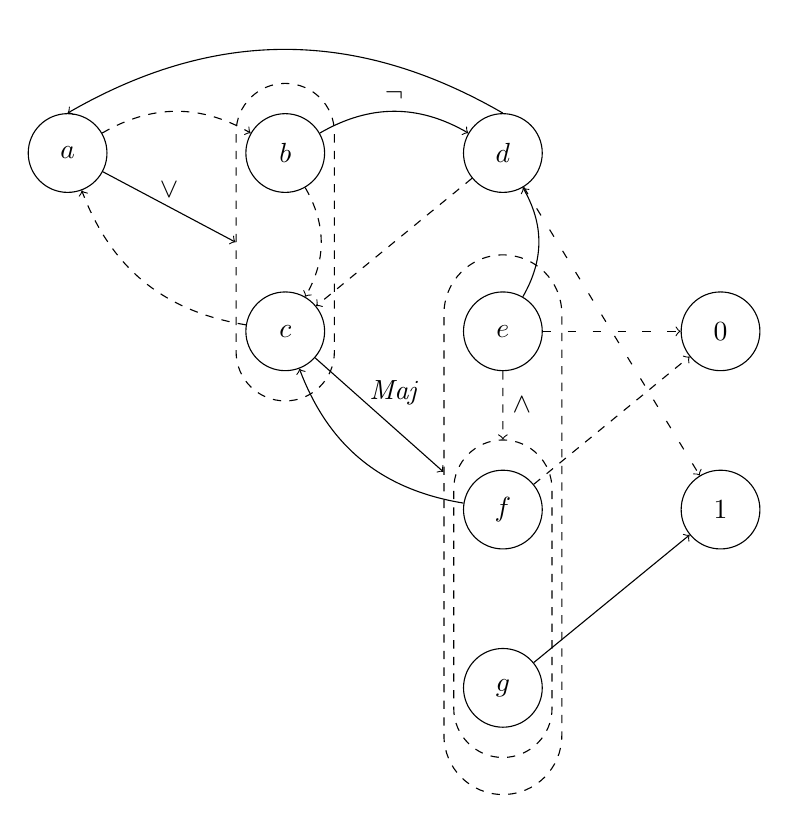
\begin{tikzpicture}
        \tikzset{node distance=1.25cm and 1.75cm}
    
        \node[circ] (a){$a$};
        
        \node[circ, right= of a](b) {$b$};
        \node[circ, below= of b](c) {$c$};

        \node[circ, right= of b](d) {$d$};
        
        \node[circ, right= of c](e) {$e$};
        \node[circ, below= of e](f) {$f$};
        \node[circ, below= of f](g) {$g$};

        \node[circ, right= of e](zero) {0};
        \node[circ, below = of zero](one){1};

 %       \node[circ, below = of c](one'){1};
%        \node[circ, left= of one'](zero'){0};

        \node[draw,  dashed, rounded rectangle, rotate fit = 90, fit={(b)(c)}](elli_bc) {};

        \node[draw, dashed, rounded rectangle, rotate fit = 90, fit={(f)(g)}](elli_fg) {};
        \node[draw, dashed, rounded rectangle, rotate fit = 90, fit={(f)(g)(e)(elli_fg)}](elli_fge) {};

        \draw[->](a) to node[midway,above] {$\lor$} (elli_bc.north);
        \draw[->, dashed](a) to [bend left] (b);
%        \draw[->, loosely dashed] (a) to (zero');

        \draw[->] (b) to [bend left] node[midway,above] {$\neg$}(d);
        \draw[->, dashed] (b) to [bend left] (c);
 %       \draw[->, loosely dashed] (b) to [bend right] (one');


        \draw[->] (c) to node[midway,above, xshift = 2mm] {$\Maj$}(elli_fge);
        \draw[->, dashed] (c) to [bend left] (a);
  %      \draw[->, loosely dashed] (c) to (zero');

        \draw[->] (d.north) to [bend right] (a.north);
        \draw[->, dashed] (d) to (c);
        \draw[->, loosely dashed] (d) to (one);

        \draw[->, dashed] (e) to node[midway,right] {$\land$}(elli_fg);
        \draw[->] (e) to [bend right] (d);
        \draw[->, loosely dashed] (e) to (zero);

        \draw[->] (f) to [bend left] (c);
        \draw[->, dashed] (f) to (zero);

        \draw[->] (g) to (one);

        
    \end{tikzpicture}
    \caption{An example of a smart profile}
    \label{fig:example}
\end{figure}


Throughout this work it will be meaningful to restrict the functions agents can delegate from. The most notable classes of functions we will consider are: 

\begin{itemize}
    \item Direct delegations to voter $v$ denoted by $\mathit{LIQUID} = \{\mathit{id}_v \mid v \in N\}$, where $\mathit{id}_v$ is the identity function applied to the vote of voter $v$.
    \item Boolean functions in disjunctive normal form denoted by $\mathit{BOOL}$. 
    \item Monotone boolean function in disjunctive normal form denoted by $\mathit{MON}$-$\mathit{BOOL}$.
\end{itemize}


\subsection{Unravellings}

Now that we have defined each agent's preferences we need to formalise how to make sense of these preferences. To do so, we use \emph{unravelling procedures} to determine each agent's vote.

\begin{definition}[Unravelling Procedure]
    An \emph{unravelling procedure} is any computable function $\mathcal{U}$ where $\mathbf{B} \mapsto^\mathcal{U} \vec{d}$ with $\vec{d} \in D^n$.
\end{definition}

The reason we need to consider unravelling procedures is that smart ballots can create cycles.
Different choices on how to ``unravel'' cycles will produce different outcomes.
For the majority of this work we will focus on the mathematical and computational properties of different unravelling procedures.


When the outcome is calculated, it is important for agents to know which preference level was used to compute their vote. 
To do so we introduce the notion of a certificate:

\begin{definition}[Certificate]
    A \emph{certificate} $\mathbf{c} \in \mathbb{N}^n$ for a profile $\mathbf{B}$ is a vector where for each $a \in N$ such that $B_a = (B_a^0 > \ldots > B_a^{k_a})$, the entry $c_a \in [0, k_a]$ corresponds to the preference level for agent $a$.  
\end{definition}


Something that will be of high importance is that functions of interest can be calculated on partial input.  
For example, consider majority rule denote as $\mathit{Maj}$. For a variable $a$, $\mathit{Maj}(1, 1, a)$ will always resolve to 1 regardless of agent $a$'s vote. 
We refer to these cases as \emph{necessary winners} as in \citet{konczak2005voting}.
We formalise this in the following definition where we use $\Delta$ to denote placeholder values.

\begin{definition}[Necessary winners]
    Let $F \colon D^n \longrightarrow D $ be a function.
    We define the \emph{necessary winner extension} $F' \colon \left\{D \cup \left\{\Delta\right\}\right\}^n \longrightarrow D \cup \left\{\Delta\right\}$ of function $F$. 
    We set for all $\vec{d} \in D^n$, $F'(\vec{d}) = F(\vec{d})$.
    For $\vec{d} \in \left\{D \cup \left\{\Delta\right\}\right\}^n$, let $i_1, i_2, \ldots, i_m$ be the indices such that $d_{i_j} = \Delta$.
    Let $\vec{d}[x_1, \ldots, x_m]$ denote the vector $\vec{d}$ where $x_j$ replaces the value at index $i_j$. Then, if for some $y \in D$ and for all $\vec{x} \in D^m$, $F(\vec{d}[\vec{x}]) = y$ then $F'(\vec{d}) = y$.
    Otherwise $F'(\vec{d}) = \Delta$.
\end{definition}

To actually use our agents' preferences we need to introduce the concept of a consistent certificate. 
Consistent certificates are certificates where the vote of each agent is determined by the votes of other agents using the functions in their smart ballots. Formally:

\begin{definition}[Consistent certificate]
    For a profile $\mathbf{B}$, a certificate $\mathbf{c}$ is \emph{consistent} if there is an ordering $\mathbf{\sigma} \colon N \longrightarrow \{1,\ldots, n\}$ of agents starting from vector $\vec{X}^0 = (\Delta, \ldots, \Delta)$ with placeholder values $\Delta$ for all agents, iteratively constructs an outcome vector of direct votes $\vec{X} \in D^n$ as follows for $\sigma(a) = z \in [1,n]$. For ease of notation we abbreviate agent $a$'s $c_a$th function, $F_a^{c_a}$ to $F$.
    \[
        X^z_a = F'(\vec{X}^{z-1} \restriction_{S^{c_a}_a} ).
    \]
    Here, $X_a$ represents agent $a$'s entry in $\vec{X}$. 
    The restriction of vector $\vec{X}$ in $S$, written as $\vec{X} \restriction_S$, is a vector indexed by $S$ where for each $s \in S$,  $(\vec{X} \restriction_S)_s = X_s$.


\end{definition}


Now, we are only interested in consistent certificates as these are the ones that respect the agents' votes. We will denote the set of consistent certificates of a profile $\mathbf{B}$ as $C(\mathbf{B})$.
It is good that there is only one outcome matched to each consistent certificate regardless of the ordering $\sigma$. The following proposition is proven by \cite{grandi}.

\begin{proposition}
    If a consistent certificate $\mathbf{c}$ can be given by two orderings $\sigma$ and $\sigma'$ of the agents, then the orderings yield the same outcome $\vec{X}_\mathbf{c} \in D^n$.
\end{proposition}

Consequently, consistent certificates are enough to determine every agent's vote. 
Now that we have settled the framework it's time to consider some ``good'' certificates. 
There is a very natural ``cost'' in this scenario and that is using a lot of the later preferences of each agent. 
So, we can set two very natural ways of minimising this cost. 
We can attempt to minimise the sum of the costs or in a more egalitarian spirit attempt to minimise the maximum cost. 
Formally:

\begin{definition}[MinSum]
    For a given profile $\mathbf{B}$, the \textsc{MinSum} unravelling procedure is defined as:
    \[
        \textsc{MinSum}(\mathbf{B}) = 
        \left\{X_{\mathbf{c}} \bigm| \mathrm{arg} \min_{\mathbf{c} \in C(\mathbf{B})} \sum_{i=1}^n c_i\right\}.
    \]
\end{definition}

\begin{definition}[MinMax]
    For a given profile $\mathbf{B}$, the \textsc{MinMax} unravelling procedure is defined as:
    \[
        \textsc{MinMax}(\mathbf{B}) = \left\{X_{\mathbf{c}} \bigm| \mathrm{arg} \min_{\mathbf{c} \in C(\mathbf{B})} \max (\mathbf{c}) \right\}.
    \]
\end{definition}

The above unravelling procedures have already been introduced and studied by  \cite{grandi}. 
A natural extension of \textsc{MinMax}, is that of \textsc{MinMaxSum} that selects from the \textsc{MinMax} certificates the ones with minimum sum. 
Formally:

\begin{definition}[MinMaxSum]
    For a given profile $\mathbf{B}$, the \textsc{MinMaxSum} unravelling procedure s defined as:
    \[
        \textsc{MinMaxSum}(\mathbf{B}) =  \left\{ X_{\mathbf{c}}\mid \arg  \min_{\vec{c} \in \mathit{minC}(\mathbf{B})} \sum_{i=1}^n c_i \right\}.
    \]
    where $\mathit{minC}(\vec{B})$ is the set of consistent certificates that minimise the maximum $c_i$. 
\end{definition}

We can apply these to our illustrative example in Figure \ref{fig:example}. We first observe that $(1, \ldots, 1)$ is not a consistent certificate. Because for an ordering $\sigma$ using only the first preferences, $\sigma(a) > \sigma(b)$ or $\sigma(a) > \sigma(c)$ as $a$ delegates to $b \lor c$. But, $\sigma(b) > \sigma(d) > \sigma(a)$. So it must be that $\sigma(a) > \sigma(c)$. But, $\sigma(c) > \sigma(f)$ or $\sigma(c) > \sigma(e)$ as $c$ delegates to the majority $\Maj(e, f, g)$. 
But $f$ delegates to $c$ so $\sigma(c) > \sigma(e)$, but again $\sigma(e) > \sigma(d)$ leading to a contradiction.

So, if there is a certificate using only the first two preferences then it is a \textsc{MinMax} certificate. 
Such a certificate is the one given by the resolving voters in the order $g < f < e < c < b < a < d$.
Where $g = 1$, $f = 0$, $e = f \land g = 0$, $c = Maj(e, f, g) = 0$, $b = c = 0$, $a = b \lor c = 0$, $d = a = 0$. This gives a certificate $\vec{c} = (1, 2, 1, 1, 2, 2, 1)$.
In fact, one can be convinced that this is a \textsc{MinMaxSum} certificate by considering all other certificates where every voter votes for their first preference except for two voters which vote for their second preference.

On the other hand a \textsc{MinSum} certificate is given by $\vec{c} = (1, 1, 3, 1, 1, 1, 1)$.
Here, $c$ votes directly for $1$. Then, $a = b \lor c = 1$, $d = a = 1$, $b = \overline{d} = 0$. Further $f = c = 1$, $e = d = 1$ and $g$ votes directly for $1$.
To verify that this is indeed a \textsc{MinSum} certificate we need to check that there is no consistent certificate $(1, \ldots, 1, 2, 1, \ldots, 1)$.
Although usually tedious, in this case the only suitable candidate would be to use the second preference of $f$ to vote for $0$ directly. But then $\Maj(e, f, g)$ cannot be resolved as $e$ is undecided. But $d, a, b$ are also undecided. So this is not a consistent certificate.
Hence, $\vec{c}$ is a consistent certificate.
Note that $\vec{c}$ is not the only \textsc{MinSum} certificate. We can select the third preference of $d$ and the first preference of other agents.
Then, we get an ordering $g < d < b < e < c < f < a$.
This is given by $d$ and $g$ voting directly for $1$.
Then, $b = \overline{d} = 0$, $e = d = 1$. So, $c = \Maj(e, f, g) = 1$, by necessary winners despite not having decided $f$. Then $f = c = 1$ and $a = b \lor c = 1$.

\newpage



\section{Complexity Results}
\label{section:Complexity}

\subsection{Hardness Results}

In order to study the computational properties of the unravelling procedures we set them up as decision problems.

\begin{definition}[\textsc{BoundedMinSum}]
    Let \textsc{BoundedMinSum}$_\mathcal{F}$ be the decision problem with input a target constant $M$ and a smart profile $\mathbf{B}$ which uses functions in the class $\mathcal{F}$. 
    The YES instances are those with a consistent certificate  $\vec{c}$ with $\sum_i c_i \leq M$. 
\end{definition}

\begin{definition}[\textsc{BoundedMinMax}]
    Let \textsc{BoundedMinMax}$_\mathcal{F}$ be the decision problem with input a target constant $M$ and a smart profile $\mathbf{B}$ which uses functions in the class $\mathcal{F}$. The YES instances are those with a consistent certificate  $\vec{c}$ with $\max(\vec{c}) \leq M$. 
\end{definition}

\begin{definition}[\textsc{BoundedMinMaxSum}]
    Let \textsc{BoundedMinMaxSum}$_\mathcal{F}$ be the decision problem with input target constants $M, S$ and a smart profile $\mathbf{B}$ which uses functions in the class $\mathcal{F}$. The YES instances are those with a consistent certificate  $\vec{c}$ with $\max (\vec{c}) \leq M$ and $\sum_i c_i \leq S$.
\end{definition}


\citeauthor{grandi} have proven that \textsc{BoundedMinSum}$_\mathit{LIQUID}$ and \textsc{BoundedMinMax}$_\mathit{LIQUID}$ are poly-time computable and that \textsc{BoundedMinSum}$_\mathit{MON\text{-}BOOL}$ and \textsc{BoundedMinMax}$_\mathit{BOOL}$ are NP-complete.
We improve on these hardness results by introducing novel gadgets and conclude some inapproximability results.

Before delving any further, we can consider the trivially easy cases. 
For any function class $\mathcal{F}$, \textsc{BoundedMinSum}$_\mathcal{F}$ and \textsc{BoundedMinMax}$_\mathcal{F}$ are trivially solvable if the maximum size of the ballot is 1. That is because every agent is required to vote for a constant.

Now, let $\lor$ be the binary logical OR and $\land$ be the binary logical AND. Then:

\begin{proposition}[Hardness of \textsc{BoundedMinSum}]
    Suppose $\mathit{LIQUID} \cup \{\lor, \land\} \subseteq \mathcal{F}$. Then \textsc{BoundedMinSum}$_\mathcal{F}$ is NP-hard, even if the maximum size of a smart ballot is 2.    
\end{proposition}

\begin{proof}
    We reduce from the NP-hard problem of \textsc{3-SAT}.
    Let $\varphi = \bigwedge_{i = 1}^k t_i $ a \textsc{3-SAT} instance on boolean variables $x_1, \ldots, x_n$ with $t_i = l_a \lor l_b \lor l_c $ where $l_a, l_b, l_c$ correspond to literals of variables $x_a, x_b, x_c$ or their negations.
    
    We first define constant voter \underline{zero}, that always votes for 0, so that $B_{\text{\underline{zero}}} = (0)$.


For each variable $x_i$ we construct a voter $x_i$ with voting profile $B_{x_i} = (  \text{\underline{zero}} > 1) $. These are drawn in Figure \ref{fig:votes}. We denote the first preferences as solid lines and second preferences as dashed lines.


We then construct gadgets for each term $t_h$. 
These gadgets will have the property that they incur no additional cost if $t_h$ is satisfied and a cost of at least one if $t_h$ is not satisfied. We prove this for the four different structures of a term $t_h$.

\begin{figure}
    \centering
    \subfloat[\underline{zero} voter]{
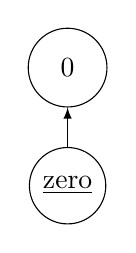
\begin{tikzpicture}[edge from parent/.style={draw,-latex}, align=center,node distance=1.75cm]

\node[circle,draw] (z){\underline{zero}} [grow = up]
    child{node [circ]{0}
    };
\end{tikzpicture}
    }
    \qquad
    \subfloat[Voter $x_i$]{
        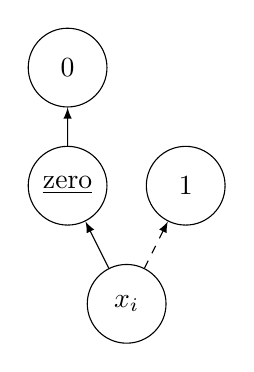
\begin{tikzpicture}[edge from parent/.style={draw,-latex}, align=center,node distance=1.75cm]

            \node[circ] (x){$x_i$} [grow = up]
            
                child{node[circ] (1){1}  edge from parent [dashed]}
                child{node [circ] (z){\underline{zero}}{
                    child{node[circ](0){0}}}
                };
            \end{tikzpicture}
    }
    \caption{Setting up the variables voters}
    \label{fig:votes}
\end{figure}

\textbf{Case} $x_i \lor x_j \lor x_k$: We construct fresh voters $t_h$, $a$, $b$, and $c$ with smart profiles:

\begin{align*}
    &B_a = (t_h > 0) \\
    &B_b = (x_i \lor a > 0) \\
    &B_c = (x_j \lor b > 0) \\
    &B_{t_h} = (x_k \lor c > 0).
\end{align*}
Now, we analyse when first preferences of the additional voters can be resolved without producing cycles. If $x_i = 1$ then $x_i \lor a = 1$ and $b$ resolves to vote $1$ using the first preference. 
Hence, $b \lor x_j = 1$ and $c$ resolves to $1$ using first preference. 
Similarly, $t_h$ resolves to $1$ and then $a$ resolves to $1$ using only first preferences. 
Similarly, if $x_j = 1$ or $x_k = 1$, agents $c$ and $t_h$ respectively will resolve to $1$ and so all fresh agents will resolve their votes using only first preferences.

Now, suppose $x_i = x_j = x_k = 0$. Suppose there is an ordering $\sigma \colon N \longrightarrow \{1,\ldots, m\}$ that gives rise to a consistent certificate using only the first preferences of agents $a, b, c, t_h$. Then, $\sigma(t_h) < \sigma(a)$ as $a$ needs $t_h$ to be resolved. Further, $\sigma(c) < \sigma(t_h)$ as $x_k = 0$ and so $c$ determines the clause $x_k \lor c$. Similarly, $\sigma(b) < \sigma(c)$ and $\sigma(a) < \sigma(b)$. This leads to the contradiction that $\sigma(a) < \sigma(a)$. Therefore, no such ordering exists and if $x_i = x_j = x_k = 0$, one of the fresh voters $a, b, c, t_h$ will need to incur a cost of at least $1$.

\textbf{Case} $\overline{x_i} \lor x_j \lor x_k$: We construct additional voters $t_h$, $a$, $b$ and $c$, with smart profiles:

\begin{align*}
    &B_a = (t_h > 0) \\
    &B_b = (x_i \land a > 0) \\
    &B_c = (x_j \lor b > 0) \\
    &B_{t_h} = (x_k \lor c > 0).
\end{align*}
This is demonstrated by Figure \ref{fig:MinSum:1nots}.

\tikzset{circ/.style={circle,draw, solid, inner sep=0pt,minimum size=10mm}}
    \begin{figure}
        \centering
    \subfloat[\centering Case $\overline{x_i} \lor x_j \lor x_k$]{{
    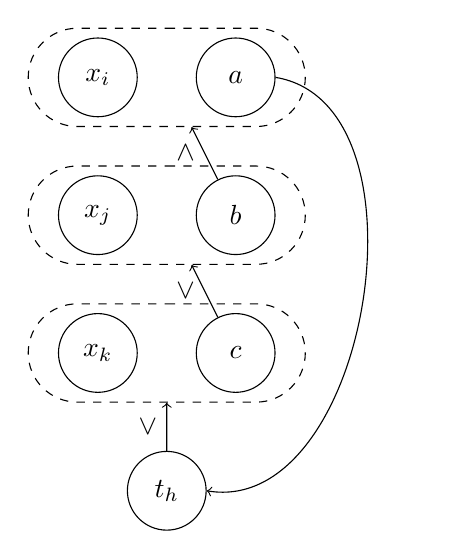
\begin{tikzpicture}[edge from parent/.style={draw,-latex}, align=center,node distance=1.75cm]
    
    \node[circ] (xi){$x_i$};
    \node[circ, right of=xi] (a){$a$};
    

    \node[circ, below of=xi] (xj){$x_j$};
    \node[circ, below of=xj] (xk){$x_k$};
    \node[circ, right of=xj] (b){$b$};
    \node[circ, right of=xk] (c){$c$};
    
    
    \node[draw, dashed, rounded rectangle, fit={(xi)(a)}] (elli1) {};
    \node[draw, dashed, rounded rectangle, fit={(b)(xj)}](elli2) {};
    \node[draw, dashed, rounded rectangle, fit={(c)(xk)}](elli3) {};

    \node[circ, below of=elli3](t){$t_h$};
    
    \draw [->] (b) -- (elli1) node[midway,left]{$\land$};
    \draw [->] (c) -- (elli2) node[midway,left]{$\lor$};
    \draw [->] (t) -- (elli3) node[midway,left]{$\lor$};
    \draw [->] (a.east) to [bend left=90] (t.east) {};
    
    \end{tikzpicture}
    \label{fig:MinSum:1nots}
    }}
    \qquad
    \subfloat[Case $\overline{x_i} \lor \overline{x_j} \lor x_k$]{{
        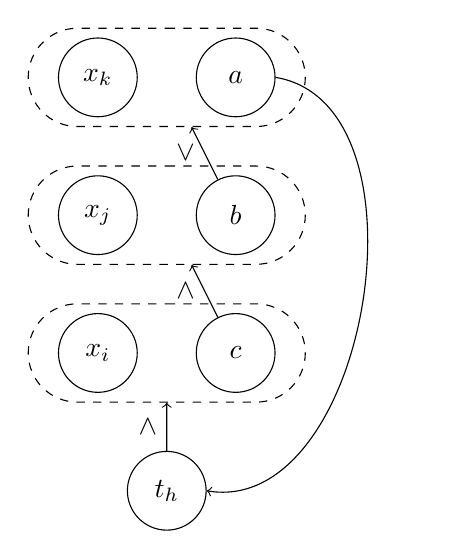
\begin{tikzpicture}[edge from parent/.style={draw,-latex}, align=center,node distance=1.75cm]
    
            \node[circ] (xk){$x_k$};
            \node[circ, right of=xk] (a){$a$};
            
        
            \node[circ, below of=xk] (xj){$x_j$};
            \node[circ, below of=xj] (xi){$x_i$};
            \node[circ, right of=xj] (b){$b$};
            \node[circ, right of=xi] (c){$c$};
            
            
            \node[draw, dashed, rounded rectangle, fit={(xk)(a)}] (elli1) {};
            \node[draw, dashed, rounded rectangle, fit={(b)(xj)}](elli2) {};
            \node[draw, dashed, rounded rectangle, fit={(c)(xi)}](elli3) {};
        
            \node[circ, below of=elli3](t){$t_h$};
            
            \draw [->] (b) -- (elli1) node[midway,left]{$\lor$};
            \draw [->] (c) -- (elli2) node[midway,left]{$\land$};
            \draw [->] (t) -- (elli3) node[midway,left]{$\land$};
            \draw [->] (a.east) to [bend left=90] (t.east) {};
            
        \end{tikzpicture}
        \label{fig:MinSum:2nots}
    }}
    \caption{Gadgets for \textsc{MinSum}}
    \label{fig:MinSum}
    \end{figure}
    
    Now, we analyse when first preferences of the additional voters can be resolved without producing cycles. 
    If $x_k = 1$ then $t_h$ can resolve to $1$ and so will $a$. 
    As $x_i$ and $a$ are set to a value, $b$ can resolve its first preference. 
    As $x_j$ and $b$ are set, $c$ can resolve its first delegation as well. 
    Similarly, if $x_j = 1$ then $c$ is immediately resolved to $1$ and so $t_h$ is resolved. 
    Hence, $a$ and then $b$ can be resolved. 
    Similarly, if $x_i = 0$ $x_i \land a = 0$ and so $b$ resolves to $0$ and all additional voters are resolved.
    
    Now, suppose $x_i = 1, x_j = 0, x_k = 0$. Then $t_h$ cannot immediately resolve the logical OR as it is dependent on the vote of $c$, similarly $c$ is waiting for $b$ to decide, and $b$ is waiting for $a$. 
    But $a$ is waiting for $t_h$ to decide. 
    There is no way to resolve this cycle, and so one of the additional voters we have introduced will have to vote for their second preference. 
    This will incur an additional cost of at least 1.

    \textbf{Case} $\overline{x_i} \lor \overline{x_j} \lor x_k$: 
    The proof is symmetrical for this case. We need to switch some ANDs to ORs and vice versa but other than that it is identical. 
    For completeness, we show the resulting gadget in Figure \ref{fig:MinSum:2nots}. 
    This is the result of a smart profile of:

    \begin{align*}
        &B_a = (t_h > 0) \\
        &B_b = (x_k \lor a > 0) \\
        &B_c = (x_j \land b > 0) \\
        &B_{t_h} = (x_i \land c > 0)
    \end{align*}

    \textbf{Case} $\overline{x_i} \lor \overline{x_j} \lor \overline{x_k}$:
    The proof is symmetrical to the case of $x_i \lor x_j \lor x_k$. We only need to switch $\lor$ to $\land$. This is achieved by the following smart ballot:
    \begin{align*}
        &B_a = (t_h > 0) \\
        &B_b = (x_i \land a > 0) \\
        &B_c = (x_j \land b > 0) \\
        &B_{t_h} = (x_k \land c > 0).
    \end{align*}
    
    Now suppose that for each term we construct $n + 1$ such gadgets for each term. Then if every term is satisfied by some assignment of the variables $x_1, x_2, \ldots, x_n$ then the total cost incurred will be at most $n$. That is because the fresh voters incur no additional cost but each voter $x_i$ can incur a cost of at most 1.
    If a term is not satisfied then at least $n+1$ gadgets will incur a cost of at least $1$ so that the cost is at least $n+1$. 
    Hence we have reduced the satisfiability of any \textsc{3-SAT} instance $\varphi$ to querying if there is a certificate $\vec{c}$ for the above election with $\sum_{i} c_i \leq n$. Thus \textsc{BoundedMinSum}$_\mathcal{F}$ is NP-hard.
\end{proof}

\begin{corollary}[Hardness of \textsc{BoundedMinMaxSum}]
    If $ \mathit{LIQUID} \cup \{\lor, \land\} \subseteq \mathcal{F}$ then \textsc{BoundedMinMaxSum}$_\mathcal{F}$ is NP-hard. 
\end{corollary}

\begin{proof}
    Every instance of \textsc{BoundedMinSum} is an instance of \textsc{BoundedMinMaxSum}. For target maximum sum $S$ and smart profile $\vec{B}$ a \textsc{MinMax} query, we can consider a \textsc{MinMaxSum} query with target maximum $M$, target sum $S$ and smart profile $\vec{B}$. Simply set $M$ to be the maximum of the size of smart ballots, i.e., $M = \max_{a \in N} k_a$. Then the max requirement of \textsc{MinMaxSum} is trivially satisfied and so we have reduced \textsc{BoundedMinMax} to \textsc{BoundedMinMaxSum}.
\end{proof}


\begin{corollary}[Inapproximability of \textsc{BoundedMinSum}] A constant factor approximation of \textsc{BoundedMinSum}$_\mathcal{F}$ is NP-hard.    
\end{corollary}

\begin{proof}
    We can adapt the above proof to prove that \textsc{BoundedMinSum} is not constant-factor approximable. 
    Following our construction above we can incur a cost of $k$ for when the expression $\varphi$ is not satisfiable by simply creating $k$ gadgets for each term. 
    So for a \textsc{MinSum} outcome $\vec{c}$:   $\sum_i c_i \leq n$ if and only if $\varphi$ is satisfiable and $\sum_i c_i \geq k$ if and only if $\varphi$ is not satisfiable. 
    So, any constant factor approximator would solve \textsc{3-SAT}, thus proving hardness.
\end{proof}

Now we shift our focus on \textsc{BoundedMinMax}.
We first note that there is an additional easiness lemma for \BMM.
The point of this lemma is that \BMM\ does not introduce any additional hardness beyond the hardness needed for computing the necessary winner of a function.

\begin{proposition}
    Let $\mathcal{F}$ be any computable family of functions and $\vec{B}$ a smart profile where each ballot has size at most 2.
    Suppose for each function $f \in \mathcal{F}$, the necessary winner $f'$ can be computed in time $T$.
    Then, there is an algorithm that decides $\BMM_\mathcal{F}$ which runs in $\mathcal{O}(n^2\cdot T)$ steps. 
\end{proposition}

\begin{proof}
    Let $m_i$ the size of the ballot of agent $i$, as always $\vec{c} = (m_1, \ldots, m_n)$ is a consistent certificate, as each delegate votes for a constant.
    As each $m_i \leq 2$, the only possible certificate that improves on $\vec{c}$ is $\vec{1} = (1, \ldots, 1)$.
    To check if $\vec{1}$ is consistent, we first set all agents $a$ with $F_a^1$ constant and equal to $d$ to $d$.
    Then, we check iteratively if any of the unset agents can vote using their first preference.
    We repeat this step until running this iteration makes no changes.
    We return that $\vec{1}$ is a consistent certificate if and only if all agents are set at this final point.

    We now prove correctness of the above.
    If the algorithm returns that $\vec{1}$ is a consistent certificate then it truly is so. 
    It can be proved by constructing $\sigma \colon N \longrightarrow \{1,\ldots, n\}$ where $\sigma(a)$ is the position in which $a$ was activated by our algorithm.
    By our definition, $a$ then uses only the values of agents that were set before $a$ in this ordering.
    Now consider every case where $\vec{1}$ is a consistent certificate with a corresponding ordering $\sigma$.
    Then, without loss of generality all the agents that vote for constants are placed first in positions $1, \ldots, k$.
    Then, for $\sigma(a) = k+1$, $F_a^{1}$ can be calculated using only agents $v$ with $\sigma(v) \leq k$, hence our algorithm will set $a$ to vote for $F_a^1$. Inductively, it will reconstruct an equivalent ordering to $\sigma$.

\end{proof}

Now that we have the easiness result the following hardness result will be tight.
Our construction is similar to the one for \BMS.
Instead of using multiple gadgets to amplify the effect of cycles we create some additional cycles by introducing primed voters $a', b', c' \text{ and } t_h'$.

\begin{proposition}[Hardness of \textsc{BoundedMinMax}]
    Suppose $\mathit{LIQUID} \cup \{\lor, \land\} \subseteq \mathcal{F}$. Then \textsc{BoundedMinMax} is NP-hard, even if the maximum size of a smart ballot is 3.    
\end{proposition}

\begin{proof}
    We follow a similar construction as above. We reduce from the NP-hard problem \textsc{3-SAT}. Suppose $\varphi$ is an instance of \textsc{3-SAT} as above on $k$ terms and $n$ variables. We again introduce constant voter \underline{zero} with smart ballot $B_{\text{\underline{zero}}} = (0)$. For each variable $x_i$ we create a voter $x_i$ with smart ballot $B_{x_i} = (\text{\underline{zero}} > 1)$. For each term $t_h$ we create gadgets with the property that if $t_h$ is satisfied the gadget uses only the first two preference levels. If $t_h$ is not satisfied, the gadget uses the third preference level. We prove this for the following four cases.

    \textbf{Case} $t_h = x_i \lor x_j \lor x_k$:
    For each term we construct additional voters $a, a', b, b', c, c', t_h$. With voting profiles: 
    \begin{align*}
        &B_a = (a' > t_h > 0) \\
        &B_{a'} = (a > t_h > 0) \\
        &B_{b} = (b' > x_i \lor a > 0) \\
        &B_{b'} = (b > x_i \lor a > 0) \\
        &B_{c} = (c' > x_j \lor b > 0) \\
        &B_{c'} = (c > x_j \lor b > 0) \\
        &B_{t_h} = (t_h' > x_k \lor c > 0) \\
        &B_{t_h'} = (t_h > x_k \lor c > 0).
    \end{align*}

    Now, we claim that if $t_h$ is satisfied then this component can be resolved with at most the second preference being used. 
    If $x_k = 1$ then we can resolve $t_h, t_h'$ to $1$ using their second preferences. 
    Hence, we can then resolve agents in order $(a, a', b, b', c, c')$ using the agents' second preference. 
    Similarly if $x_j = 1$ we can resolve in order $(c, c', t_h, t_h', a, a, b, b')$ using only the agents' first two preferences. Similarly, for $x_i = 1$.

    Now consider the case where $x_i = x_j = x_k = 0$. Let $\sigma \colon N \longrightarrow \{1, \ldots, m\}$ be an ordering of the $m$ agents from which a consistent certificate arises. Suppose, this only uses the agents' first two preferences.
    As the fresh agents $a, b, c, t_h$ are identical with the primed versions $a', b', c', t_h'$, without loss of generality every unprimed agent appears before their primed counterpart so for instance $\sigma(t_h) < \sigma(t_h')$. 
    Then, $\sigma(c) < \sigma(t_h)$ as $x_k \lor c$ cannot be resolved with $x_k = 0$. 
    Similarly, $\sigma(b) < \sigma(c)$ and $ \sigma(a) < \sigma(b)$ but $\sigma(t_h) < \sigma(a)$. This leads to the contradiction $\sigma(t_h) < \sigma(t_h)$. 
    Hence, if $t_h$ is not satisfied, one of the fresh agents will use their third preferences, and if $t_h$ is satisfied, all fresh agents will use only their first two preferences.

    \textbf{Case} $t_h = \overline{x_i} \lor x_j \lor x_k$:
    For each term we construct additional voters $a, a', b, b', c, c', t_h$. With voting profiles: 
    \begin{align*}
        &B_a = (a' > t_h > 0) \\
        &B_{a'} = (a > t_h > 0) \\
        &B_{b} = (b' > x_i \land a > 0) \\
        &B_{b'} = (b > x_i \land a > 0) \\
        &B_{c} = (c' > x_j \lor b > 0) \\
        &B_{c'} = (c > x_j \lor b > 0) \\
        &B_{t_h} = (t_h' > c \lor x_k > 0) \\
        &B_{t_h'} = (t_h > c \lor x_k > 0).
    \end{align*}

    We present this smart ballot in the much easier to parse Figure \ref{fig:MinMax:1nots} where solid lines indicate first preferences and dashed lines indicate second preferences:
\tikzset{circ/.style={circle,draw, solid, inner sep=0pt,minimum size=10mm}}
    \begin{figure}
        \centering

    \subfloat[\centering Case $\overline{x_i} \lor x_j \lor x_k$]{{
    \begin{tikzpicture}[edge from parent/.style={draw,-latex}, align=center,node distance=1.75cm]
    
    \node[circ] (xi){$x_i$};
    \node[circ, right of=xi] (a){$a$};
    \node[circ, right of=a] (a'){$a'$};    

    \node[circ, below of=xi] (xj){$x_j$};
    \node[circ, right of=xj] (b){$b$};
    \node[circ, right of=b] (b'){$b'$};
    
    \node[circ, below of=xj] (xk){$x_k$};
    \node[circ, right of=xk] (c){$c$};
    \node[circ, right of=c] (c'){$c'$};
    
    \node[circ, below of=elli3](t){$t_h$};
    \node[circ, right of=t](t'){$t_h'$};

    \node[draw, dashed, rounded rectangle, fit={(xi)(a)}] (elli1) {};
    \node[draw, dashed, rounded rectangle, fit={(b)(xj)}](elli2) {};
    \node[draw, dashed, rounded rectangle, fit={(c)(xk)}](elli3) {};


    
    \draw [->] (a) to [bend right] (a');
    \draw [->] (a') to [bend right] (a);
    \draw[->, dashed] (a) .. controls (-3, 4) and (-2, -7) .. (t);
    \draw[->, dashed] (a') .. controls (5, -2) and (5, -5) .. (t');


    \draw[->] (b) to [bend right] (b');
    \draw[->] (b') to [bend right] (b);
    \draw [->, dashed] (b) -- (elli1) node[midway,left]{$\land$};
    \draw [->, dashed] (b') -- (elli1) node[midway,right]{$\land$};

    \draw[->] (c) to [bend right] (c');
    \draw[->] (c') to [bend right] (c);
    \draw [->, dashed] (c) -- (elli2) node[midway,left]{$\lor$};
    \draw [->, dashed] (c') -- (elli2) node[midway,right]{$\lor$};
    

    \draw[->] (t) to [bend right] (t');
    \draw[->] (t') to [bend right] (t);
    \draw [->, dashed] (t) -- (elli3) node[midway,left]{$\lor$};
    \draw [->, dashed] (t') -- (elli3) node[midway,right]{$\lor$};
    
    \end{tikzpicture}
    }
    \label{fig:MinMax:1nots}
    }
    \subfloat[\centering Case $\overline{x_i} \lor \overline{x_j} \lor x_k$]{{
        \begin{tikzpicture}[edge from parent/.style={draw,-latex}, align=center,node distance=1.75cm]
    
            \node[circ] (xk){$x_k$};
            \node[circ, right of=xk] (a){$a$};
            \node[circ, right of=a] (a'){$a'$};    
        
            \node[circ, below of=xk] (xj){$x_j$};
            \node[circ, right of=xj] (b){$b$};
            \node[circ, right of=b] (b'){$b'$};
            
            \node[circ, below of=xj] (xi){$x_i$};
            \node[circ, right of=xi] (c){$c$};
            \node[circ, right of=c] (c'){$c'$};
            
            \node[circ, below of=elli3](t){$t_h$};
            \node[circ, right of=t](t'){$t_h'$};
        
            \node[draw, dashed, rounded rectangle, fit={(xk)(a)}] (elli1) {};
            \node[draw, dashed, rounded rectangle, fit={(b)(xj)}](elli2) {};
            \node[draw, dashed, rounded rectangle, fit={(c)(xi)}](elli3) {};
        
        
            
            \draw [->] (a) to [bend right] (a');
            \draw [->] (a') to [bend right] (a);
            \draw[->, dashed] (a) .. controls (-3, 4) and (-2, -7) .. (t);
            \draw[->, dashed] (a') .. controls (5, -2) and (5, -5) .. (t');
        
        
            \draw[->] (b) to [bend right] (b');
            \draw[->] (b') to [bend right] (b);
            \draw [->, dashed] (b) -- (elli1) node[midway,left]{$\lor$};
            \draw [->, dashed] (b') -- (elli1) node[midway,right]{$\lor$};
        
            \draw[->] (c) to [bend right] (c');
            \draw[->] (c') to [bend right] (c);
            \draw [->, dashed] (c) -- (elli2) node[midway,left]{$\land$};
            \draw [->, dashed] (c') -- (elli2) node[midway,right]{$\land$};
            
        
            \draw[->] (t) to [bend right] (t');
            \draw[->] (t') to [bend right] (t);
            \draw [->, dashed] (t) -- (elli3) node[midway,left]{$\land$};
            \draw [->, dashed] (t') -- (elli3) node[midway,right]{$\land$};
            
            \end{tikzpicture}
    }}
    \caption{Gadgets for \textsc{MinMax}}
    \end{figure}

    Now, we claim that if $t_h$ is satisfied then this component can be resolved with at most the second preference being used. 
    If $x_k = 1$ then we can resolve $t_h, t_h'$ to $1$ using their second preferences. 
    Hence, we can then resolve agents in order $(a, a', b, b', c, c')$. 
    Similarly, if $x_j = 1$ we can resolve in order $(c, c', t_h, t_h', a, a, b, b')$ using only the agents first two preferences. 
    Now, if $x_i = 0$ the same argument holds, as the logical AND is resolved to 0. 

    Now consider the case where $x_i = 1, x_j = 0$ and $x_k = 0$. Let $\sigma \colon N \longrightarrow \{1, \ldots, m\}$ be an ordering of the $m$ agents from which a consistent certificate arises. Suppose, this only uses the agents' first two preferences.
    As the fresh agents $a, b, c, t_h$ are identical with the primed versions $a', b', c', t_h'$, without loss of generality every unprimed agent appears before their primed counterpart, so for instance $\sigma(t_h) < \sigma(t_h')$. 
    Then, $\sigma(c) < \sigma(t_h)$ as $x_k \lor c$ cannot be resolved with $x_k = 0$. 
    Similarly, $\sigma(b) < \sigma(c)$. Again, $ \sigma(a) < \sigma(b)$ as $x_i \land a = a$ as $x_i = 1$. But $\sigma(t_h) < \sigma(a)$. This leads to the contradiction $\sigma(t_h) < \sigma(t_h)$. 
    Hence, if $t_h$ is not satisfied one of the fresh agents will use their third preferences and if $t_h$ is satisfied all fresh agents will use only their first two preferences.

    \textbf{Case} $\overline{x_i} \lor \overline{x_j} \lor x_k$: This case is symmetrical to the above. We only need to permute the agents and replace the logical ANDs with ORs and vice versa. For completeness, the smart voting profiles are:     \begin{align*}
        &B_a = (a' > t_h > 0) \\
        &B_{a'} = (a > t_h > 0) \\
        &B_{b} = (b' > x_k \lor a > 0) \\
        &B_{b'} = (b > x_k \lor a > 0) \\
        &B_{c} = (c' > x_j \land b > 0) \\
        &B_{c'} = (c > x_j \land b > 0) \\
        &B_{t_h} = (t_h' > c \land x_i > 0) \\
        &B_{t_h'} = (t_h > c \land x_i > 0)
    \end{align*}

    \textbf{Case} $\overline{x_i} \lor \overline{x_j} \lor \overline{x_k}$: The proof is symmetrical to the case $x_i \lor x_j \lor x_k$. The smart ballot used reverses $\lor$ to $\land$. This is accomplished by the following smart profile:

    \begin{align*}
        &B_a = (a' > t_h > 0) \\
        &B_{a'} = (a > t_h > 0) \\
        &B_{b} = (b' > x_i \land a > 0) \\
        &B_{b'} = (b > x_i \land a > 0) \\
        &B_{c} = (c' > x_j \land b > 0) \\
        &B_{c'} = (c > x_j \land b > 0) \\
        &B_{t_h} = (t_h' > x_k \land c > 0) \\
        &B_{t_h'} = (t_h > x_k \land c > 0).
    \end{align*}

    So, $\varphi$ is satisfiable if and only if there exists a consistent certificate $\vec{c}$ with $\max(\vec{c}) \leq 2$. Hence, we have reduced \textsc{3-SAT} to \textsc{BoundedMinMax}$_\mathcal{F}$, proving that \textsc{BoundedMinMax}$_\mathcal{F}$ is NP-hard.
\end{proof}

\begin{proposition}[\textsc{BoundedMinMax} is not approximable]
    If $\mathit{LIQUID} \cup \{\lor, \land\} \subseteq \mathcal{F}$ then a non-trivial approximation of \textsc{BoundedMinMax}$_\mathcal{F}$ is NP-hard.
\end{proposition}

\begin{proof}
    This result can be proven by modifying the above proof. Instead of constructing a cycle of size 2 for voters $a, b, c, t_h$, we construct a cycle of size $k + 1$. So every voter $a, b, c, t_h$ can be thought of as a voter $v$ with $B_v = (v' > u > 0)$. Then we construct voters $v_1, \ldots, v_k$ and set $B_v = (v_1 > v_2 > \ldots > v_k > u > 0)$ and for $v_i$, $B_{v_i} = (v > v_1 > \ldots > v_{i - 1} > v_{i+1} > \ldots > v_k > u > 0)$.
    Now, since the maximum size of the smart ballots is $k + 2$ then clearly for the \textsc{MinMax} certificate $\vec{c}$, $\max{\vec{c}} \leq k + 2$. 
    But suppose that an algorithm was able to decide if there was $\vec{c}$ with $\max{\vec{c}} \leq k + 1$. Then this algorithm would be able to determine if the original instance is satisfied. So, it would solve \textsc{3-SAT}.
\end{proof}

\subsection{Extensions of Hardness}

Throughout this process we have proven results for $\lor$ and $\land$.
We can use these results to prove that hardness results extend to all ``reasonable" and sufficiently complex function classes.
We make this precise below.
First, we consider that ``reasonable'' functions are monotone. 
We define $0 < 1$ and extend this to a partial order in $\{0,1\}^n$ as $\vec{u} \leq \vec{v}$ if for all $i$, $u_i \leq v_i$.
Then we can define monotonicity of a function.

\begin{definition}[Monotonicity]
    \label{monotonicity}
    Function $f\colon \{0, 1\}^n \longrightarrow \{0, 1\}$ is \emph{monotone} if for all $\vec{u}, \vec{v} \in \{0,1\}^n$, $\vec{u} \leq \vec{v}$ implies that $f(\vec{u}) \leq f(\vec{v})$.
\end{definition}

We also, need to be able to refer to functions that are not equivalent to direct delegation. 
These functions are referred to as dictator functions by \cite{boolean} and are equivalent to projection functions.

\begin{definition}[Dictator functions]
    Function $f \colon \{0, 1\}^n \longrightarrow \{0, 1\}$ is a \emph{dictator function} if there is some index $1 \leq i \leq n$ such that for every $\vec{x} \in \{0, 1\}^n$, $f(\vec{x}) = x_i$.
\end{definition}

\begin{lemma}
    \label{lem:boolean}
    Let $f \colon \{0,1\}^n \longrightarrow \{0,1\}$ for $k \geq 2$, be a function that is monotone, non-constant and not a dictator function.
    Then there exist indices $i, j$ with $i < j$ and constants $c_k$ for $1 \leq k \leq n$ and $k \neq i$ and $k \neq j$ such that $f(c_1, \ldots, c_{i-1}, x_i, c_{i+1}, \ldots, c_{j-1}, x_j, c_{j+1}, \ldots, c_n) = x_i \lor x_j$ or $x_i \land x_j$.
\end{lemma}

\begin{proof}
    By \cite{boolean} exercise 4.3, any monotone function $f$ can be written as a boolean formula in disjunctive normal form \emph{without negations}.
    Let $f(\vec{x}) = \bigvee_{i = 1}^k t_i$, with $t_i = x_{j_1} \land \ldots \land x_{j_r}$.
    Without loss of generality we can assume that for all $i$ and $j$, $t_i \nrightarrow t_j$.
    Then, $k \geq 1$ as $f$ is not constant.
    
    Suppose $t_1 = x_{j_1} \land \ldots \land x_{j_r}$ for $j_r > 1$. 
    Then, we can pick $j_1, j_2$ as distinguished indices. Set $c_{j_i} = 1$ for $i > 2$ and $c_i = 0$ otherwise.
    So that for $i > 1$, terms $t_i$ evaluate to $0$ and $t_1 =x_{j_1} \lor x_{j_2}$.
    Hence, $f$ is equivalent to $x_{j_1} \land x_{j_2}$.
    
    If $t_1 = x_j$, then as $f$ is not a dictator, $k > 1$.
    As $t_1 \nrightarrow t_2$, $t_2$ does not contain $x_j$.
    Hence, for $t_2 = x_i \land \varphi$ for some $\varphi$, we can set all variables of $\phi$ to 1 and all variables not appearing in $t_1$ or $t_2$ to 0.
    Then, for any $t_r$ for $r > 2$, $t_r = 0$. That is because $t_r$ cannot contain $x_j$ and the variables $t_r$ of $t_r$ cannot be a subset of the variables of $t_2$.
    So, $t_r$ contains variables not in $t_1$ and not in $t_2$ which are set to $0$. So $t_r$ is set to 0.
    Hence, $f$ is made equivalent to $x_i \lor x_j$.
\end{proof}

Now, we need a final ingredient to add to our conditions for reasonable functions to discuss function classes.
We think that it is reasonable that agents are offered functions of similar expressibility regardless of voting in favour of 0 or 1.
For instance, if qualified majorities in favour of 0 are allowed then we would expect in most scenarios that qualified majorities in favour of 1 to be allowed.
This concept can be formalised by considering the dual of each function as stated in \cite{boolean}.

\begin{definition}[Duality]
    Let $f \colon \{0, 1\}^n \longrightarrow \{0, 1\}$. Then $f$'s dual function $f^\dagger \colon \{0, 1\}^n \longrightarrow \{0, 1\}$ defined as $f^\dagger(\vec{x}) = \overline{f(\overline{\vec{x}})}$.
\end{definition}

In particular $\lor^\dagger = \land,\Maj^\dagger= \Maj$ and for $\Maj_k^0$ the qualified majority of $k$ in favour of $0$, $(\Maj_k^0)^\dagger = \Maj_k^1$.

So, we would expect that in most settings the choices of voters to be closed under taking duals.
Nevertheless, the following key theorem works even if there is only one sufficiently ``complex'' but monotone function $f$ and the dual $f^\dagger$.

\begin{theorem}
    Let $\mathcal{F}$ any function class such that $\mathcal{F}$ contains $\LIQUID$. Suppose $f, f^\dagger \in \mathcal{F}$ with $f$ non-constant, not dictatorial and monotone.
    Then $\BMS_\mathcal{F}$ and $\BMMS_\mathcal{F}$ are NP-hard even if the maximum ballot size is 2. $\BMM_{\mathcal{F}}$ is NP-hard even if the maximum ballot size is 3.
\end{theorem}

\begin{proof}
    By Lemma \ref{lem:boolean} there are designated indexes $i, j$ and constants $c_k$ for $k \neq i, j$ such that $f$ is equivalent to $x_i \lor x_j$ or to $x_i \land x_j$.
    Hence, for constants $\overline{c_k}$, $f^\dagger$ is equivalent to $x_i \lor x_j$ if $f$ is equivalent to $x_i \land x_j$ or vice versa.
    Hence, by constructing suitably many constant voters \underline{zero} and \underline{one} with $B_{\text{\underline{zero}}} = (0)$ and $B_{\text{\underline{one}}} = (1)$, $f$ and $f^\dagger$ can be used to simulate $\lor$ and $\land$.
    Hence, our propositions of hardness hold here as well.
\end{proof}

As an immediate corollary, if agents are allowed to delegate to some odd majority then \textsc{MinSum} and \textsc{MinMax} are NP-hard.
This resolves the question left open in \citet{grandi}.

\subsection{Results for $\LIQUID$}

Now that we've shown hardness results for function classes larger than $\LIQUID$ we focus on what we can do with $\LIQUID$.

For every smart ballot $\vec{B}$ with delegating functions from $\LIQUID$ we can construct a directed graph that encodes this information $\varphi(\vec{B})$. In $\varphi(\vec{B})$ every arborescence is a valid certificate of the election induced by $\vec{B}$. As a reminder, an arborescence $A$ in a directed graph $G = (V, E)$ rooted in $r$ is a subgraph for which for each $u \in V \setminus \{r\}$  there exists a unique path from $r$ to $u$. This construction is essentially in \citet{grandi} and we formalise it below.

For an election with voters $N$ and smart ballot $\vec{B}$, we construct $\varphi(\vec{B}) = (V, E)$ as follows.
For $V = N \cup \{0, 1, r\}$ where $0, 1$ and  $r$ are fresh nodes. For each voter $v \in N$ with smart ballot $B_v = (a_1 > \ldots > a_k)$ for $ 1 \leq i \leq k$ we construct edges $(a_i, v)$.
In addition, we construct edges $(r, 0), (r, 1)$.
Then we can claim that:

\begin{proposition}
    For every smart profile $\vec{B}$ there is a natural bijection between the consistent certificates of $\vec{B}$ and the arborescences of $\varphi(\vec{B})$ rooted in $r$. This is given by having voter $v$ delegate to their parent in the arborescence.
\end{proposition}

\begin{proof}
    Let $A$ an arborescence of $\varphi(\vec{B})$ rooted in $r$.
    Let voter $v$ delegate to their parent $\mathrm{par}(v)$.
    Then every agent is delegating to a unique agent by the properties of the arborescence.
    Additionally, there are no cycles and every chain of delegations reaches $0$ or $1$ as they are the only vertices that are children of the root, so every voter is a assigned a vote.

    In the other direction let $\vec{c}$ a consistent certificate. 
    Let $d \colon N \longrightarrow N \cup\{0, 1\}$ the delegation function induced by $\vec{c}$.
    Then, $(d(u), u)$ forms are arborescence.
    That is because for every voter $u$ there is a unique path to a constant symbol.
\end{proof} 
This construction allows us to argue graph-theoretically about $\LIQUID$ elections.

Consider the problem of finding a \textsc{MinMax} certificate on instances with $n$ voters and at most $l$ preference levels.
The paper by \citet{grandi} provides a $\mathcal{O}(n^2l^2)$ algorithm for finding a \textsc{MinMax} certificate. With two tweaks we construct an algorithm that runs in $\mathcal{O}(nl \log l)$.

\begin{proposition}
    Consider an instance with voters $N = \{1, \ldots, n\}$ and smart ballot $\vec{B}$. 
    Let maximum preference used by any voter is $l$.
    Then there is a $\mathcal{O}(nl \log l)$ algorithm that returns a \textsc{MinMax} certificate.
\end{proposition}

\begin{proof}
    Suppose we want to check if there exists a consistent certificate using the agents' first $m$ preferences. Then we can consider the smart ballot given by the first $m$ preferences $\vec{B}_m$.
    Then it suffices to check if there exists an arborescence of $\varphi(\vec{B}_m)$.
    To do so, we can run Depth First Search from $r$ in $\mathcal{O}(nm)$ steps. As $m \leq l$, it is $\mathcal{O}(nl)$.
    If there is an arborescence it will be returned as the DFS tree of the traversal. If not, some node is unreachable from $r$ and thus $\vec{B}_m$ has no consistent certificate.

    Now, to find the smallest $m$ for which the above is satisfied we only need to binary search suitable $m$ in $\{1, \ldots, l\}$.
    This gives a total complexity of $\mathcal{O}(nl \log l)$.

\end{proof}

The above algorithm works for cases where voters are offered more than two alternatives.
To retain the complexity of $\mathcal{O}(nl \log l)$ it suffices to assume that $d \leq n$.
We also, show that it is easy to modify the above algorithm to check if there is a valid \textsc{MinMax} certificate voting for $0$ or $1$ in polynomial time.


\begin{proposition}
    Consider an instance of a monotone aggregation rule $r$ that translates the votes of the agents to the final vote of the group. 
    Then for $d \in \{0, 1\}$ there is a $\mathcal{O}(nl \log l)$ algorithm that determines if there is a \textsc{MinMax} certificate such that the election resolves in favour of $d$ and if it exists it returns the certificate.
\end{proposition}

\begin{proof}

    For ease of notation we assume without loss of generality that $d = 0$.
    We first determine by the previous algorithm the smallest $m$ for which there exists a \textsc{MinMax} certificate using at most $m$ preferences.
    Then we construct the graph $\varphi(\vec{B}_m)$.
    Then, instead of initiating a DFS search from the root we initiate it from node $0$.
    This returns the directly connected component of $0$ denoted $S$.
    Let $\vec{x}$ with $x_i = 1$ if and only if $i \in S$.
    Any voter outside of $S$  cannot be made to vote for $0$, so that $S$ is maximal. As $r$ is monotonic, if and only if  there is a possible way of resolving the election to $0$ $r(\vec{x})$ will be equal to 0.

    If $r(\vec{x}) = 1$ then we return that every valid \textsc{MinMax} outcome votes for 1.
    Otherwise, we run DFS from $1$ on the subgraph not visited by our previous DFS.
    From this we recover a valid certificate from the rest of the agents.
    We only need to return this certificate to conclude the algorithm.
    The complexity is inherited by the algorithm to determine $m$ and it is $\mathcal{O}(nl \log l)$.
\end{proof}

The above result implies that there need to be clear and predetermined rules on tie-breaking of results.
That is because it is computationally cheap to adversarially break ties to rig the election in someone's favour.

We have not been able to develop an algorithm or a proof of hardness for a similar result in \textsc{MinMaxSum}.
But, we have been able to reduce it to a graph theoretic problem in the case of qualified majorities.
A qualified majority is a rule where outcome $1$ is selected if and only if at least $k$ voters vote for $1$.

The equivalent graph theoretic question is, for graph $\varphi(\vec{B})$ is there a minimum weight arborescence with the size of subtree of $1$ greater than $k$? We leave whether this is polynomial time computable or NP-hard as an open question.

\newpage
\section{Axiomatisation}
\label{section:axioms}

We introduce the axiom of cast participation. This axiom states that voters preferring outcome $d$ benefit from voting directly for $d$. 
As mentioned in the introduction, this axiom is introduced by \cite{kotsialou} and \cite{grandi} have applied it for binary issues with abstentions. 
We use the definition for binary issues with abstentions i.e., $D = \{0, 1, *\}$.
We denote that agent $a$ prefers outcome $d$ to $e$ as $d >_a e$. As in \citeauthor{grandi} we infer that if agent $a$ votes directly for outcome $d \in \{0, 1\}$ then agent $a$ prefers $d$ over any other outcome. 
Formally if $B_a = (d)$ then $ d >_a 1-d$ and $d >_a *$.
Additionally, we consider that if agent $a$ votes directly for $d$ then $* >_a 1-d$. 
Originally, \citeauthor{kotsialou} focus on resolute unravelling procedures. \citeauthor{grandi} do so as well and only examine the axioms for their resolute heuristics.
We will extend these to the irresolute unravelling procedures we have studied.
So, we need to extend the original definition. 
We need to assign preferences over sets of outcomes rather than just for single outcomes.
For the case $D = \{0, 1, *\}$ we posit that reasonable extensions of the order $1-d <_a * <_a d$ would include the partial order:

\[
    \{1-d\} < \{1-d, *\} < \{*\} \sim \{1-d, d\} \sim \{1-d, *, d\} < \{*, d \}< \{d\}.
\]
Here $S_1 \sim S_2$ denotes that $S_1$ is not comparable to $S_2$.
Then we can formalise cast participation for irresolute procedures:

\begin{definition}[cast participation for irresolute procedures]
    A resolute voting rule $r$ and a irresolute unravelling procedure $\mathcal{U}$ satisfy cast participation if for all valid smart profiles $\mathbf{B}$ and agents $a \in N$ such that $B_a \in D \setminus \{*\}$ we have that for all $B_a' \neq B_a$:
    \[
        r(\mathcal{U}(\mathbf{B})) \geq_a r(\mathcal{U}(\mathbf{B}_{-a}, B_a')).
    \]
    Here $\mathbf{B}_{-a}, B_a'$ denotes replacing $B_a$ with $B_a'$ and $r$ is applied to subsets of $S \subseteq D^n$ as follows: $r(S) = \{r(\vec{d}) \mid \vec{d} \in S\}$.
\end{definition}

Cast participation can be thought of as disallowing tactical voting. Unfortunately, it is not always satisfied. 
We first consider the cases of some non-monotone $r$ and non-monotone delegating functions. 
Note that we have defined monotonicity for binary issues in \cref{monotonicity}. 
We extend this to issues with abstentions by considering $D = \{0, 1, *\}$ to be totally ordered as $0 < * < 1$.
Then, we can define a partial order on $D^n$ where $\vec{u} \leq \vec{v}$ if for all $i$, $u_i \leq v_i$. Then monotonicity is defined identically.

We now prove a series of negative results for cast participation.



\begin{proposition} Suppose that the voting rule $r$ is not monotone. Additionally, the counterexample to monotonicity is not caused by flipping a $*$ to a $0$ or $1$. 
That is, there exists $\vec{u} = (u_1, \ldots, u_{i-1}, 0, u_{i+1}, \ldots, u_n)$ and $\vec{u}' = (u_1, \ldots, u_{i-1}, e, u_{i+1}, \ldots, u_n)$ with $0 \neq e$ but $r(\vec{u}) > r(\vec{u}')$. 
Then cast participation does not hold.
\end{proposition}

\begin{proof}
    Consider the smart profile where for each agent $a$, $B_a = (u_a)$. 
    In particular $0 >_i * >_i 1$. We are allowed to deduce this because $i$ does not vote for an abstention.
    But, by setting a smart ballot of $B_i = (e)$ we obtain $r(\vec{u}') < r(\vec{u}')$. So voter $i$ prefers to vote directly for $e$ than $d$ despite preferring outcome $d$.
    This violates cast participation.
\end{proof}

We consider that most reasonable unravelling procedures will not needlessly violate their agents' first preferences. 
We formally say that $\mathcal{U}$ respects first preferences if whenever $\vec{c} = (1, 1, \ldots, 1)$ is a consistent certificate, $\mathcal{U}$ returns an outcome with certificate $\vec{c}$. 
Note that $\textsc{MinMax}$, $\textsc{MinSum}$ and $\textsc{MinMaxSum}$ respect first preferences as well as any Pareto optimal unravelling procedure. A notable exception is the BFS algorithm proposed by \citeauthor{kotsialou} as shorter delegation chains are preferred over longer delegation chains.

\begin{proposition}
    Suppose $r$ is a monotone rule, $\mathcal{U}$ respects first preferences. Suppose additionally, that for some $n$ and $k > 0$ there exists a ``deciding'' subset of voters $S$ with $\abs{S} \leq n - k$ such that if every voter in $S$ votes for $d$, $r$ votes for $d$.
    Then, cast participation does not hold.
\end{proposition}

\begin{proof}
    Let $S$ as defined above and $f: \{0, 1, *\}^k \longrightarrow \{0,1, *\}$.
    Further, suppose there exist $\vec{u} < \vec{u}'$ with only $u_i < u_i'$, $u_i = 0$ and $f(\vec{u}) > f(\vec{u}')$. Then, enumerate voters $v_1, \ldots, v_k$ not in $S$ and let $B_{v_i} = (u_i)$. 
    For all other agents $a$ set $B_{a} = (f(v_1, \ldots, v_k) > d)$ for some arbitrary $d$. 
    Then the first preferences of the voters do not introduce cycles. 
    As $\mathcal{U}$ respects first preferences it picks an outcome where every agent votes for their first preference.
    Hence, $r$ resolves to vote for $f(\vec{u})$ as all voters in $S$ vote for $f(\vec{u})$.
    Now if agent $v_i$ were to switch their vote from $0$ to $u_i'$ everyone in $S$ would vote for $f(\vec{u}')$ and so $r$ would resolve to $f(\vec{u}')$. This breaks cast participation for voter $v_i$ as they prefer outcome 0 but are better not voting for 0.
\end{proof}

\begin{proposition}
    \label{prop:cast-max}
    Let $r$ be a rule such that for $n \geq 5$ voters if $n-2$ voters vote for $d$ then $r$ assigns $d$. Then there are examples that unravelling with \textsc{MinMax} violates cast participation for any $n$. This result holds even if we only allow agents to vote using LIQUID.
\end{proposition}

\begin{proof}
    Let $N = \{v, v', a, u_1, \ldots, u_{n-3}\}$ and $r$ as described. Then, let $B_v = (0), B_{v'} = (v > 0), B_a = (1), B_{u_i} = (a > 0)$. Then \textsc{MinMax} would simply assign each individual to first preferences and the majority votes for 1. So the outcome set is $\{1\}$.

    But, if $B_v = (v' > 0)$ then a cycle is formed and so necessarily, \textsc{MinMax} will have to use some second preferences. Hence, setting $v, u_1, \ldots, u_{n-3}$ to their second preference would be a valid solution. So every voter except $a$ vote for $0$, so that $r$ resolves to $0$. 
    Note that we can still assign first preference to all voters except than $v$ so that $(2, 1, \ldots, 1)$ is a consistent certificate and would result to the majority again voting for 1. 
    Therefore, the set of outcomes is $\{0, 1\}$ which is better than $\{1\}$ for agent $a$.
\end{proof}

Do note that the above counterexample works even when consider issues with binary outcomes without abstentions.
Additionally, the above proof would not work in the case of \textsc{MinMaxSum}, as \textsc{MinMaxSum} would only return the certificate $(2, 1, \ldots, 1)$.

We can further prove that \textsc{MinSum} does not satisfy cast participation in general.

\begin{proposition} \label{prop:cast-sum}
    Let $r$ be such that if a strict majority votes for outcome $d$ then $r$ supports outcome $d$. Then even if we consider only binary issues, cast participation doesn't hold for \textsc{MinSum}. 
\end{proposition}

\begin{proof}
    Let $N = \{a, b, c, d, e, f, \text{\underline{zero}}\}$. Let $B_\text{\underline{zero}} = (0), B_a = (1), B_b = (\text{\underline{zero}} > 1), B_c = (a \lor b > d > 1), B_d = (a \lor b > c > 1), B_e = (b > 1)$ and $B_f = (b > 1)$. Then, the unique \textsc{MinSum} outcome is everyone voting for their first preferences with $a \lor b$ resolving to $1$ and $a, c, d$ voting for 1 and $\text{\underline{zero}}, b, e, f$ voting for 0. This gives an outcome set of $\{0\}$.

    Now, if $a$ were to switch their vote to $(c > d > 1)$, then the \textsc{MinSum} outcome set would be $\{1\}$. Because if $b$ votes for $1$ directly, every other first preference can be resolved.
    Hence, $a$ should not vote directly for 1 even though it is their preferred outcome. This violates cast participation.
\end{proof}

Note, that in the above case $\lor$ is a monotone rule. So, it is not the case that monotone rules guarantee cast participation for \textsc{MinSum} even for binary issues.

\textbf{Conjecture:}
    Suppose that $r$ is a monotone rule and voters are restricted to casting $\LIQUID$ ballots. Then \textsc{MinSum} satisfies cast participation.

\newpage
\section{Conclusion}

In summary, we have extended the work of \citet{grandi} in two directions. On the complexity theoretic level, we have produced a new hardness criterion using novel gadgets. Additionally, we have improved on the algorithms to find \textsc{MinMax} outcomes and given an algorithm that returns if a \textsc{MinMax} outcome for a particular alternative exists.
On the axiomatisation direction we have extended the definition by \citeauthor{grandi} and proved several negative results.

There are three ideas that could guide future work. First, the two open questions we leave at the end of Sections \ref{section:Complexity} and \ref{section:axioms} can be resolved. In particular, I am slightly surprised the question at the end of Section \ref{section:Complexity} has not been resolved yet, as it is a general result concerning arborescences.
Another direction is to extend the model by allowing agents to assign cardinal values of how much they approve of their preferences, instead of just ordering them.
The cardinal voting model seems like a meaningful generalisation of the preferential voting model we have here.
Finally, our hardness result implies that for many reasonable functions optimal unravellings can be NP-hard.
But there is a case relevant to the real world that is not covered by the hardness result.
One implementation of liquid democracy requires agents to choose before the election if they want to be delegated to.
Thus splitting the electorate between voters who cannot be delegated to and delegates who can be delegated to. 
Suppose we allow voters to delegate to a single boolean functions of delegates. 
But, delegates can only delegate directly to other delegates, then NP-hardness does not arise.
That is because the only cycles that need to be resolved happen in $\LIQUID$ which can be optimally unravelled in polynomial time.
This gives voters a lot of expressive power while maintaining polynomial time unravellings. 
A question that seems interesting in this setting is when it would be better for someone to join the delegates or the voters in different instances.

In these final paragraphs, I include my personal reflections.
This project has allowed me to explore a topic in detail that I was interested in before.
Initially, I was quite ambitious and tried to come up with a game-theoretic model that rewarded amassing power.
This is a reflection of real-life politics, as successful political parties get funding and members of parliament are paid a salary from the government.
As far as I have seen, such a model has not appeared in the literature yet.
The resulting model was complex and unwieldy and had no pure strategy Nash Equilibria.
Hence, we moved on to another idea where voters want to coordinate on how to delegate to delegates in order to maximise the probability of voting for the ground truth.
This path also did not yield substantial results. Nevertheless, I did come up with some nice simulations and graphs.

The direction of my work changed when my supervisor suggested I read the paper by \citet{grandi} which she thought left open questions I could answer.
I did so, and it turned out she was correct.
The paper had a wide gap between what was proven to be easy, the simplest class of functions, and hard, arbitrary boolean functions.
A class of functions that was noted throughout the work but not assigned a complexity class was that of delegating to majorities.
I grappled with this over the Christmas vacation and realised that it was indeed NP-hard.
The next task I had in mind was to check a less expressive function class that is binary OR and binary AND.
As shown in the main hardness reduction, these too turned out to be NP-hard.
I was very excited to present these to my supervisor as these superseded my previous result.

Our work would include all the complexity results but importantly, we also considered the axiomatic results in \citet{grandi}.
The axiomatic results were only for resolute procedures and so there was space to extend them to irresolute ones.
We picked the most unassuming definition we could and then started proving negative results for non-monotone functions.
I was under the impression that \textsc{MinMax} and definitely \textsc{MinSum} would satisfy cast participation for monotone functions.
It turned out I was wrong even for a restricted class of monotone functions. 
In fact, I arrived at the example of Proposition~\ref{prop:cast-sum} by trying to prove its negation.

Overall, I have deeply enjoyed the repeated successes and failures of research. 
I am quite happy with the final result which would not be possible without the guidance of my supervisor. 


\newpage
\bibliographystyle{plainnat}
\bibliography{thesis-bib.bib}
\end{document}

